% Attention:
% 1. Please use the XeLaTeX compiler, otherwise there might be issues with Chinese character compilation.
% 2. The entire document uses the Microsoft YaHei font. Ensure it is installed, or substitute with other fonts.

% Document Class Definition
% Specifies the document class using a custom Beamer class file located relative to this file.
\documentclass{../../../Cls/SDU/Beamer/Beamer}

% Load Custom Styles
% Includes custom styles defined in the Beamer.sty file, located relative to this file.
\usepackage{../../../Styles/SDU/Beamer/Beamer}

% --- Document Information Setup ---
% Sets the metadata for the presentation.

% Title setup: [Short title for footer] {Full title for title page}
\title[Beamer Template]{A Beamer Template} 
% Subtitle for the title page
\subtitle{Subtitle}
% Author's name
\author{Arshtyi}
% Institute information: [Short name for footer] {Full details for title page}
\institute[SDU] 
{   
	CS\\ % Department or affiliation
	\medskip % Adds a small vertical space
	\textit{\url{arshtyi_trantor@outlook.com}} % Email address, typeset in italics
}
% Date of the presentation, \today inserts the current date
\date{\today}

% --- Automatic Table of Contents Generation ---
% Automatically inserts a table of contents frame at the beginning of each section.

\AtBeginSection[] % Hook executed at the beginning of each \section
{
	\begin{frame}{Contents} % Start a new frame titled "Contents"
		\transfade % Apply fade transition effect (if defined in the theme/style)
		% Display table of contents, highlighting current section/subsection
		\tableofcontents[sectionstyle=show/shaded,subsectionstyle=show/shaded/hide] 
		\addtocounter{framenumber}{-1}  % Prevent ToC frames from incrementing the total frame count
	\end{frame}
}

% --- Document Body ---
% The main content of the presentation starts here.
\begin{document}

% --- Title Page Frame ---
\begin{frame}
    % Uncomment the following lines to set a background image for the title page.
    % \pgfdeclareimage[width=\paperwidth,height=0.9575\paperheight]{bg}{Images/bg.png}
    % \setbeamertemplate{background canvas}{\pgfuseimage{bg}} 
    % Uncomment for fade transition effect on the title page.
    % \transfade 
    \titlepage % Command to generate the title page based on the document information provided above.
\end{frame}

% --- Optional Initial Table of Contents ---
% You can uncomment this section if you want a table of contents right after the title page.
% \begin{frame}{Contents}  
%     % \transfade % Apply fade transition effect
%     \tableofcontents % Display the table of contents
% \end{frame}

% --- Section 1: Text Examples ---
\section{Text section} % Start of a new section

% Frame demonstrating bibliography citations
\begin{frame}
    \frametitle{The reference example} % Set the title for this frame
    \begin{itemize}
        \item The references are used as follows:
              \begin{itemize}
                  % Example of citing a reference using \footfullcite (requires biblatex)
                  \item In the article\footfullcite{8549396}, the author proposed a new algorithm.
                  \item In order to do something, article\footfullcite{6655873} designed the example protocol.
                  \item Someone\footfullcite{7307234} used the example algorithm to address the problem.
              \end{itemize}
    \end{itemize}
\end{frame}

% Frame demonstrating mathematical formula referencing
\begin{frame}
    \frametitle{The example of formula reference} % Set the title for this frame
    \begin{itemize}
        \item The reference of formula is as follows:
              \begin{itemize}
                  \item $x={r_1,r_2,\cdots,r_N}$, find the optimal solution:
                  \item thus the $P2$:
                        % Example of an aligned equation with a manual tag
                        \begin{align*} % Use align* for unnumbered equation block
                            \mathcal {P}_2: & \min \limits _{x \in \mathcal {X}} \max ({r_1, \ldots, r_N}) \tag{8} % Manual tag (8)
                        \end{align*}
              \end{itemize}
        \item this is a random sentence:
              \begin{itemize}
                  \item $H={h:X→Q}$, where $Q$ is the optimal solutions.
                  \item $S_0={(x_0,y_0),\cdots,(x_U,y_U)},$
              \end{itemize}
    \end{itemize}
\end{frame}

% --- Section 2: Image Examples ---
\section{Image section} % Start of a new section

% Frame demonstrating mixed text and image layout using columns
\begin{frame}
    \frametitle{The example of mixed text and image} % Set the title for this frame

    \begin{columns}[T] % Use columns environment, T aligns tops of columns
        % Left column for text (65% width)
        \begin{column}{.65\textwidth}
            \begin{itemize}
                \item Item1
                      \begin{itemize}
                          \item Item1.1 This is a randomly generated sentence
                          \item Item1.2 This is a randomly generated sentence
                          \item Item1.3 This is a randomly generated sentence
                      \end{itemize}
                \item Item2
            \end{itemize}
        \end{column}% % The '%' prevents extra space between columns		
        \hfill% % Horizontal flexible space, pushes columns apart	
        % Right column for image (40% width)
        \begin{column}{.40\textwidth}
            \begin{figure}[htpb] % Figure environment
                \centering % Center the image
                % Resize image to fit column width, maintaining aspect ratio
                \resizebox{1\linewidth}{!}{
                    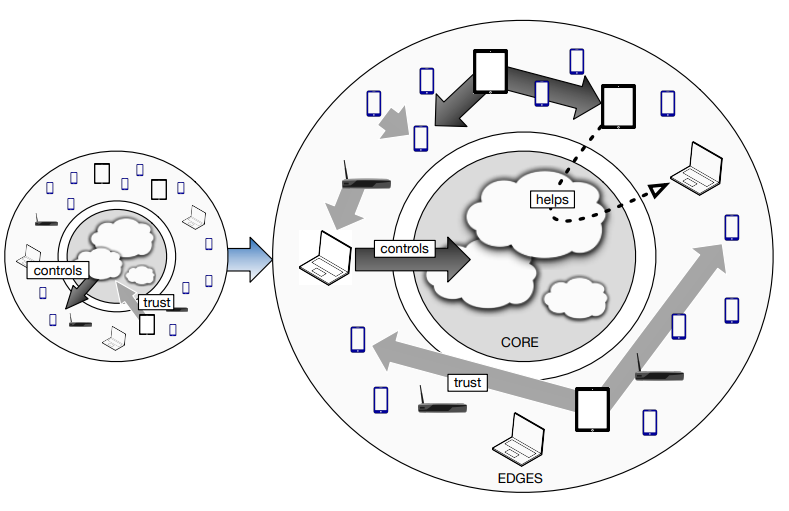
\includegraphics[scale=1.0]{Images/edge.png} % Include the image
                }
                \caption{Centralized cloud model (left) versus Edge-centric Computing (right).} % Image caption
                \label{fig:edge} % Label for referencing the figure
            \end{figure}
        \end{column}% % The '%' prevents extra space
    \end{columns}
\end{frame}

% Frame demonstrating mixed formula and image layout using columns
\begin{frame}{The example of combining formula and image} % Frame title set directly
    \begin{columns}[T] % Use columns environment, T aligns tops
        % Left column for formulas/text (65% width)
        \begin{column}{.65\textwidth}
            \begin{itemize}
                \item index set of tasks as $\mathcal{N} \triangleq\{1,2, \ldots, N\}$
                \item the index set of edge servers as $\mathcal{M} \triangleq\{1,2, \ldots, M\}$
                \item We denote the indicator of a task latency in burst load as $I^{\dagger }_i(t)$. While $I^{\dagger }_i(t) = 1$  means waiting.
                      \begin{itemize}
                          \item The latency time of the ith task denoted as:
                                % Unnumbered equation using equation* environment
                                \begin{equation*}
                                    T_1^i = \sum _{t>0} I^{\dagger }_i(t), \tag{1} % Manual tag (1)
                                \end{equation*}
                      \end{itemize}
            \end{itemize}
        \end{column}% % The '%' prevents extra space		
        \hfill% % Horizontal flexible space	
        % Right column for image (40% width)
        \begin{column}{.40\textwidth}
            \begin{figure}[thpb] % Figure environment
                \centering % Center the image
                % Resize image to fit column width
                \resizebox{1\linewidth}{!}{
                    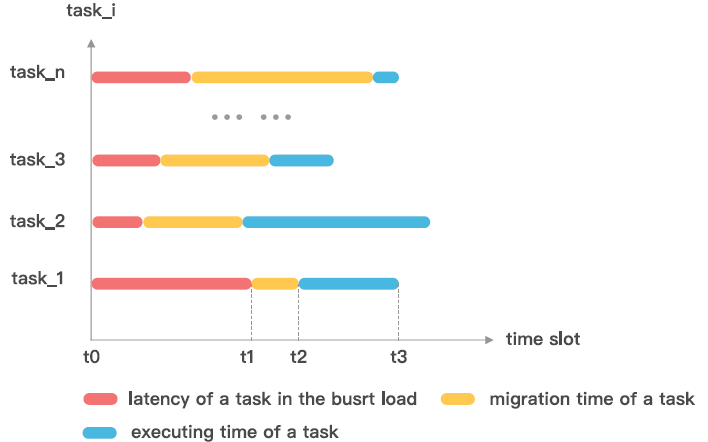
\includegraphics{Images/tasks.png} % Include the image
                }
                % Alternative way to include image with scaling:
                % \includegraphics[scale=1.0]{figurefile} 
                \caption{The flowchart of tasks when evacuation} % Image caption
                \label{fig:tasks} % Label for referencing
            \end{figure}
        \end{column}% % The '%' prevents extra space
    \end{columns}
\end{frame}

% Frame demonstrating two side-by-side images using subfigure (requires subcaption package, likely included in style)
\begin{frame}{The example of two images} % Frame title set directly
    \begin{figure}[htb] % Figure environment
        % \centering % Optional centering for the whole figure block
        \label{fig:example} % Label for the main figure environment (optional)
        % First subfigure (left)
        \begin{subfigure}{.45\textwidth} % Subfigure takes 45% of text width
            \centering % Center content within subfigure
            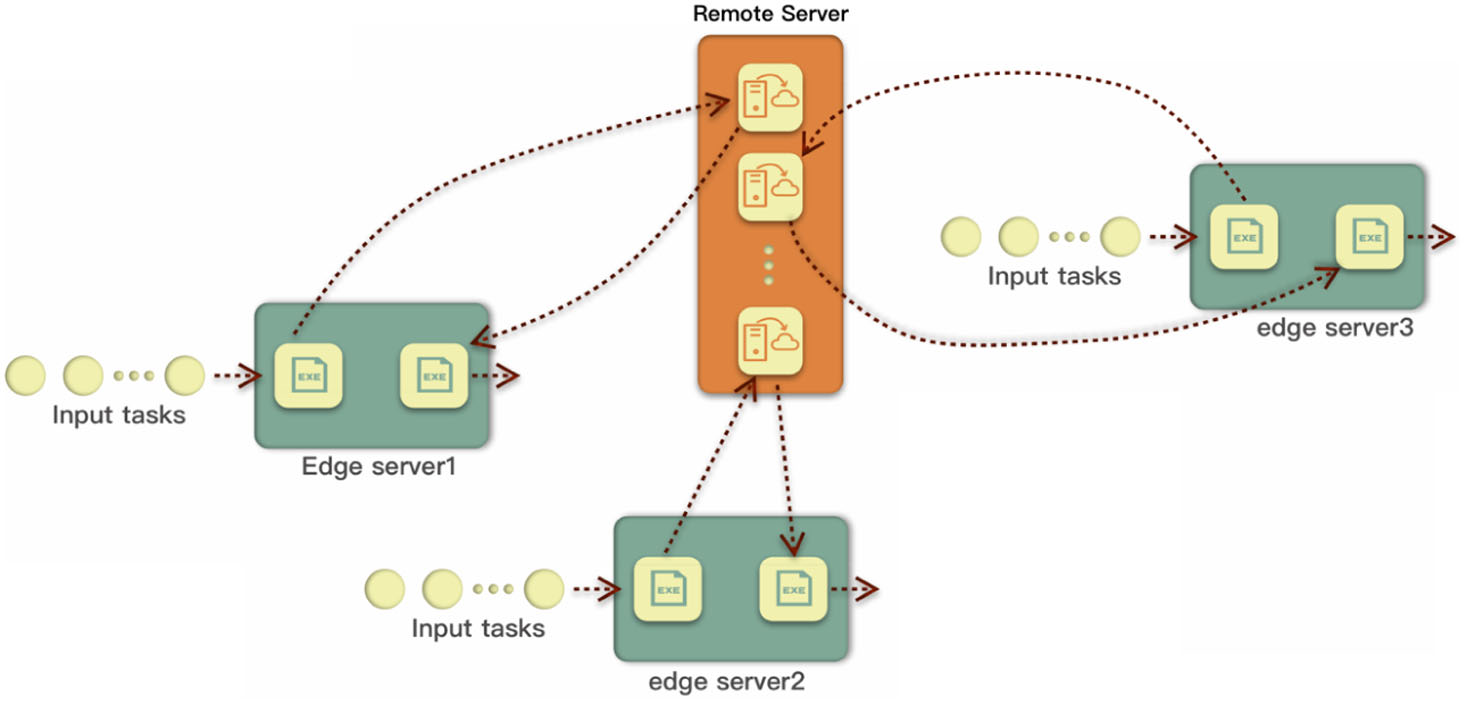
\includegraphics[width=\textwidth]{Images/scheduling.jpg} % Image scaled to subfigure width
            \caption{Task scheduling for executing and requesting data} % Subfigure caption
            \label{fig:scheduling} % Label for subfigure
        \end{subfigure}
        \hfill % Add space between subfigures
        % Second subfigure (right)
        \begin{subfigure}{.45\textwidth} % Subfigure takes 45% of text width
            \centering % Center content within subfigure
            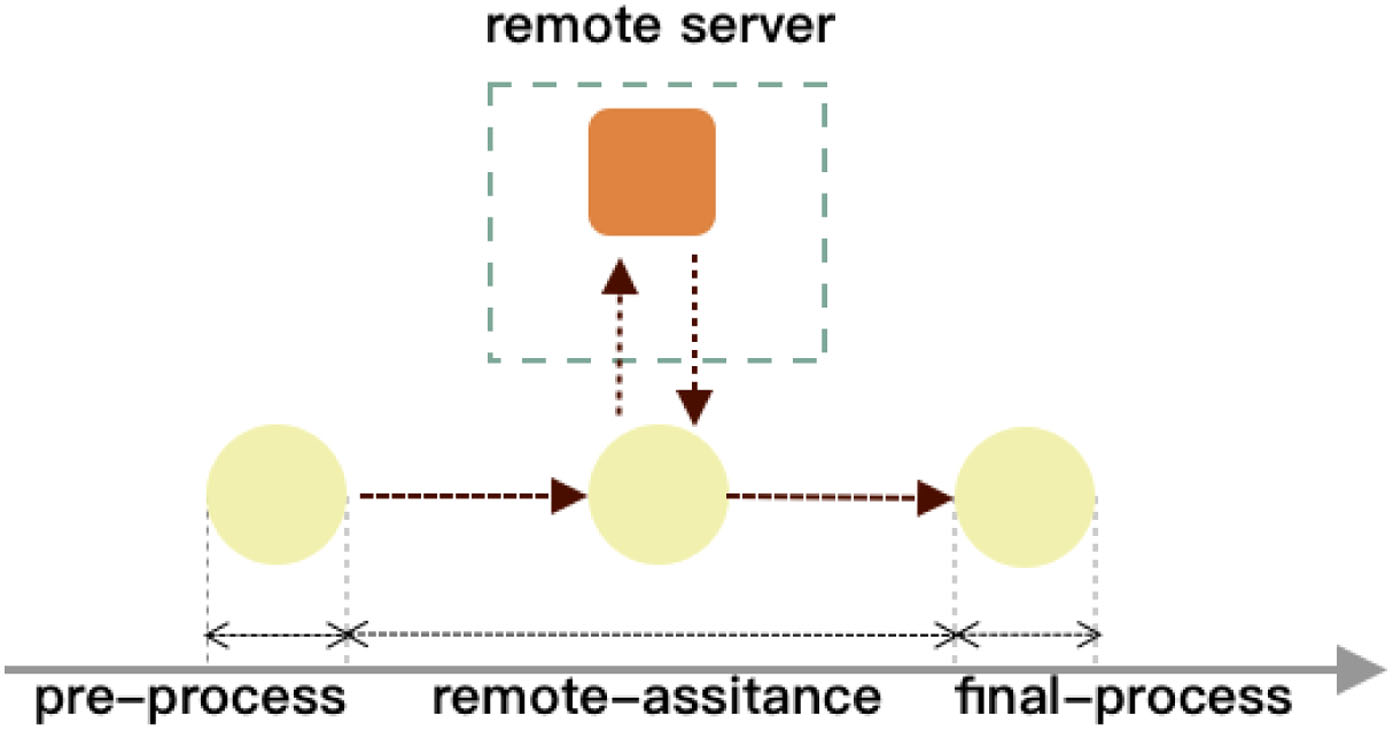
\includegraphics[width=\textwidth]{Images/processing.jpg} % Image scaled to subfigure width
            \caption{Task processing sequence.} % Subfigure caption
            \label{fig:logob} % Label for subfigure
        \end{subfigure}
        % \note{note:} % Optional note for the frame
    \end{figure}
\end{frame}

% Frame demonstrating a single centered image
\begin{frame}
    \frametitle{The example of single image} % Set the title for this frame

    \begin{figure}[htpb] % Figure environment
        \centering % Center the figure
        { % Braces for local scope if needed, not strictly necessary here
            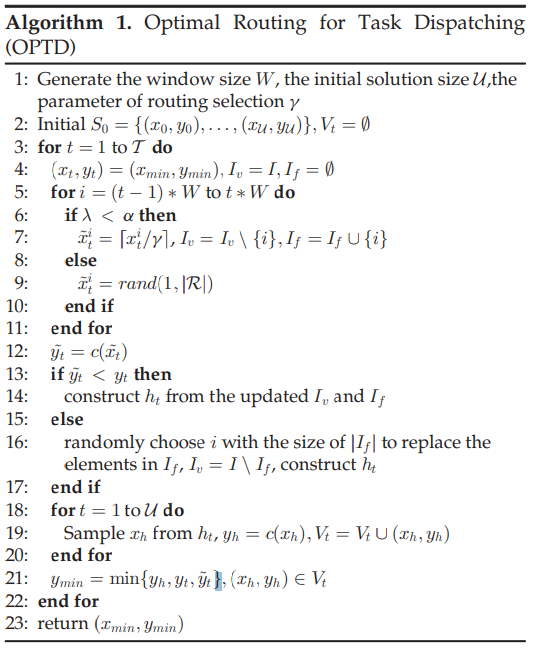
\includegraphics[scale=0.3]{Images/algorithm1.png} % Include image, scaled down
        }
        \label{fig:algorithm1} % Label for referencing
    \end{figure}

\end{frame}

% --- Bibliography Frame ---
% Displays the bibliography/references.
\begin{frame}
    \frametitle{Reference} % Set the title for this frame
    \printbibliography % Command to print the bibliography (requires biblatex/biber setup)
\end{frame}

% --- Acknowledgement Frame ---
% A final frame for acknowledgements.
\begin{frame}
    \frametitle{Acknowledgement} % Set the title for this frame
    \begin{itemize}
        \item thank y'all. % Acknowledgement text
    \end{itemize}
\end{frame}

% --- End of Document ---
\end{document}